\documentclass[12pt]{article}
\usepackage{graphicx} %package to manage images
\graphicspath{ {./figures/} }
\usepackage{caption}
\usepackage[font=scriptsize]{subcaption}
\captionsetup[figure]{labelsep=none}
\captionsetup[table]{labelsep=none}
\usepackage{bbm}
\usepackage{amsmath}
\usepackage{import}
\usepackage{array}
\usepackage{booktabs}
\usepackage{afterpage}
\usepackage{floatrow}
\usepackage{pdflscape}
\usepackage{soul}
\usepackage{float}
\usepackage{adjustbox}
\usepackage{longtable}
\usepackage{caption}
\usepackage{setspace}
\usepackage{afterpage}
\usepackage[margin=1in]{geometry}
\usepackage[round]{natbib}
\usepackage{hyperref}
\usepackage{titlesec}

\title{EGC Stata Test 070625 S278}
\date{August 7th, 2025}

\begin{document}

\maketitle


\section*{Data preparation and preliminary analysis}

\subsection*{Part 1c)}

\begin{table}[H]
    \centering
    \scriptsize % shrink text
    \setlength{\tabcolsep}{2pt}
    \renewcommand{\arraystretch}{2}
    \resizebox{\textwidth}{!}{{
\def\sym#1{\ifmmode^{#1}\else\(^{#1}\)\fi}
\begin{tabular}{l*{3}{cccccc}}
\hline\hline
            &\multicolumn{6}{c}{hhinc\_topcoded}                                           &\multicolumn{6}{c}{log\_hhinc\_topcoded}                                       &\multicolumn{6}{c}{log\_hhinc\_topcoded}                                       \\
            &        Mean&          SD&   1st pctl.&      Median&  99th pctl.&         Max&        Mean&          SD&   1st pctl.&      Median&  99th pctl.&         Max&        Mean&          SD&   1st pctl.&      Median&  99th pctl.&         Max\\
\hline
\hline
\(N\)       &        4160&            &            &            &            &            &        3916&            &            &            &            &            &        3584&            &            &            &            &            \\
\hline\hline
\multicolumn{19}{l}{\footnotesize 24-month income is estimated by 24*household income in last 30 days.}\\
\end{tabular}
}
}
    \caption{: Endline raw data summary statistics}
\end{table}

The average household in this sample earns 11,809 Rs. per month, with an average of 4.51 household members. This translates to a per-capita daily income of approximately 89.42 Rs., or 6.29 USD per day using the provided exchange rate. Though this average was well above the international threshold for extreme poverty at the time, it masks stark inequalities.

The median household income is 6,000 Rs., nearly half the mean, suggesting that most households live on modest incomes while a smaller minority earn largely more, assuming no reporting or measurement error.

Among the sample, borrowing is substantial with households having on average total formal loans of 64,382 Rs. and informal loans of 40,921 Rs., though these distributions are also skewed right and influenced by extreme upper outliers. 



Nonetheless, the amount of informal borrowing may suggests possible financial exclusion among the sample, strong informal credit networks, or a preference for informal borrowing.


\begin{figure}[H]
    \centering
    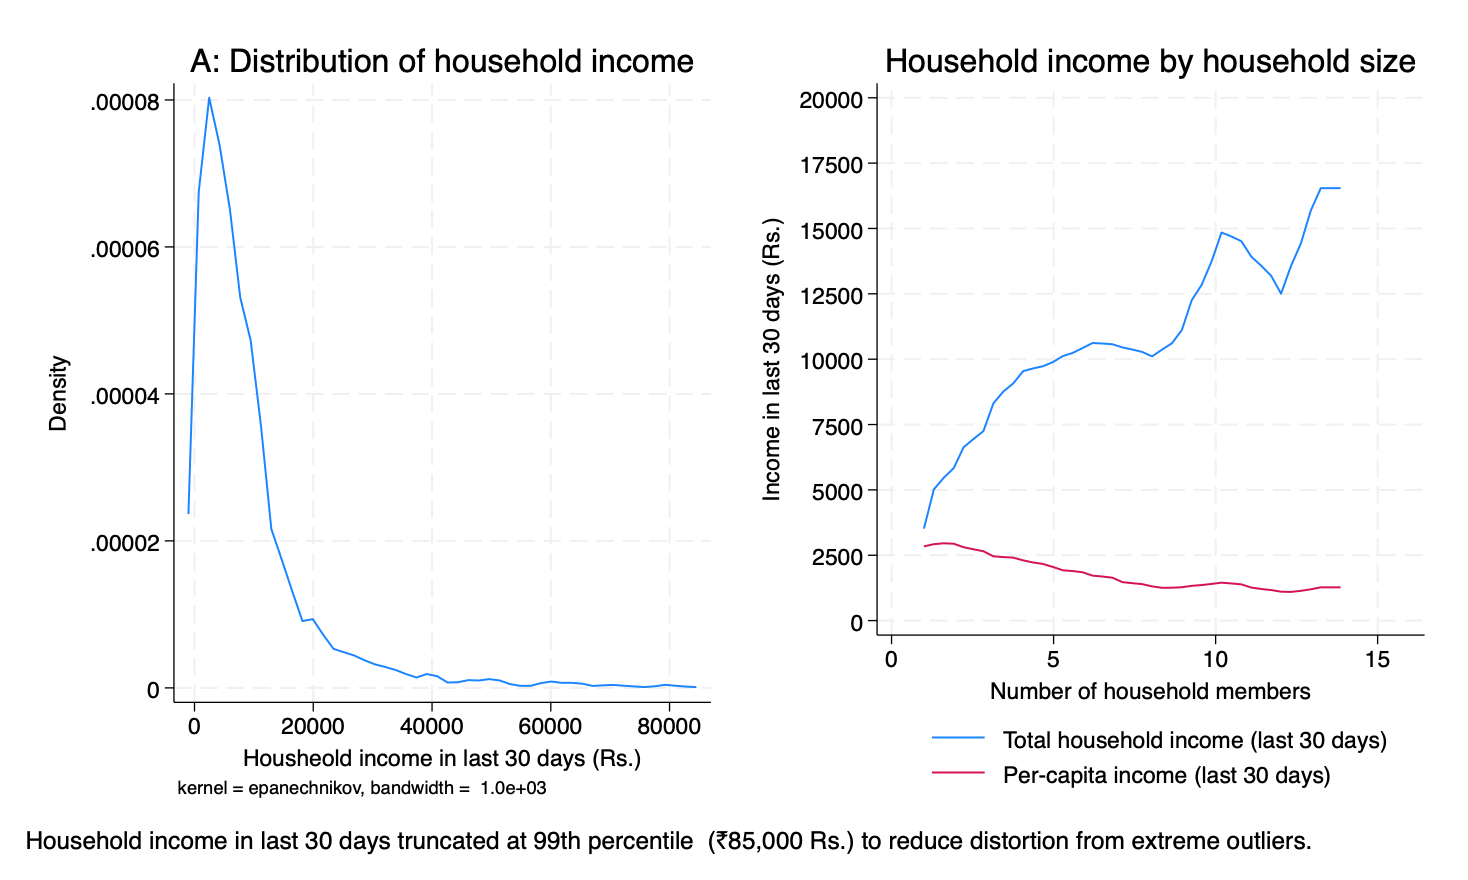
\includegraphics[width=\textwidth]{figures/figure01_hhinc.png}
    \caption{: Distribution and composition of household income in last 30 days}
\end{figure}

Panel A in figure 1 illustrates the highly right-skewed distribution of household income. Even after truncating the top 1\% of values, the kernel density plot shows that the vast majority of households earn less than 20,000 Rs. per month. Panel B illustrates that while household income was positively correlated with household size, per-capita income was negatively correlated with household size, reinforcing the importance of measuring poverty by per-capita income.


\begin{figure}[H]
    \centering
    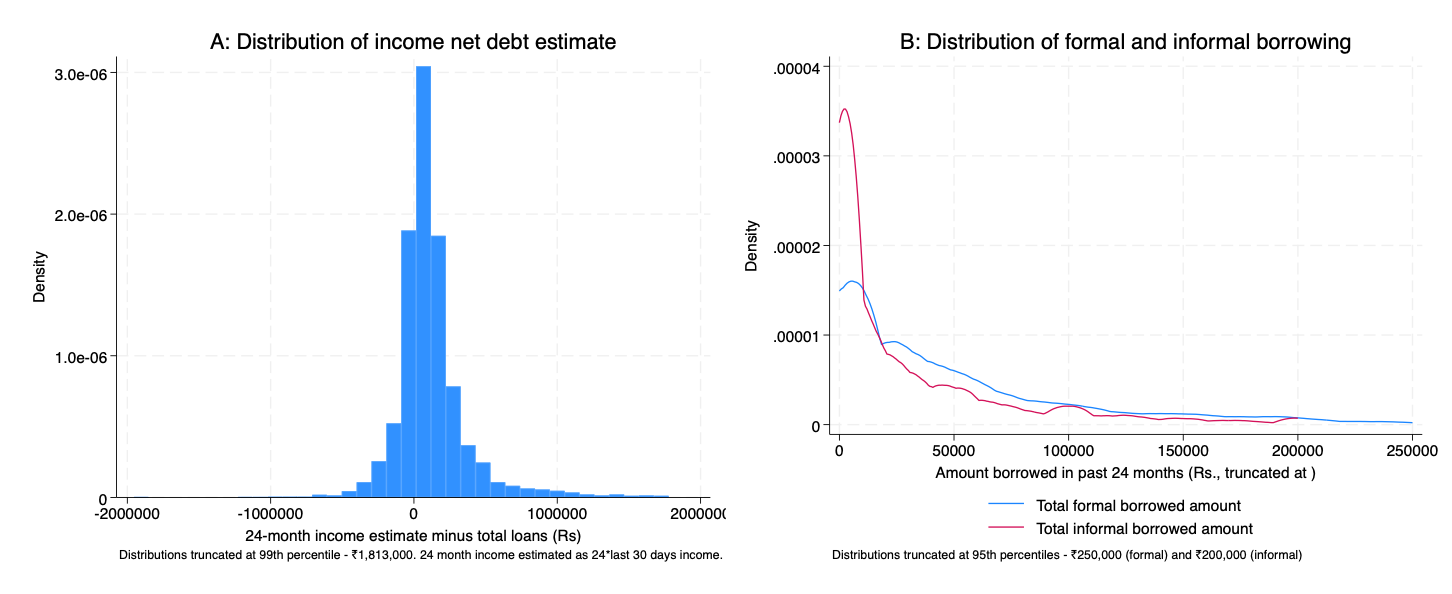
\includegraphics[width=\textwidth]{figures/figure02_loandistribution.png}
    \caption{: Distribution of total borrowing (loans) in last 24 months}
\end{figure}

Panel A in figure 2 shows the distribution of the estimate of income net debt, focusing on the bottom 99 percent of the distribution. The distribution has a tall peak centered at 0, suggesting that most households are barely accumulating financial surplus. Also, a considerable part of the distribution is below 0, suggesting high debts among the sample that may be due to expensive credit. 

Panel B in figure 2 shows that informal borrowing is far more common among the sample in smaller amounts, below around 18,000 Rs. over the last 24 months. Both distributions, like household income, are heavily skewed right. 


\subsection*{Part 1f)}

Top-coding household income and total borrowing in the last 24 months helps reduce the influence of extreme outliers that can distort summary statistics and regression estimates. In this sample, the means of these variables dropped significantly after top-coding, suggesting that the original averages were disproportionately driven by a small number of very high-income or high-debt households. Top-coding makes the analysis more representative of the broader population by limiting the influence of such extreme values.

Also, since this data is from self-reported surveys, there could be bias where people report larger incomes or borrowing than their true values for social desirability. 

Another check would be to look for instances of households having zero income with positive borrowing. This could be due to missing information or data entry errors that make these points invalid for analysis. 

\subsection*{Part 1j)}

One strength of the dummy variable for poverty (indicating households that are belowa per-capita poverty line of 26.995 INR) is that it's based on per-capita income. As we saw in figure 1 panel B, high household incomes may mask per-capita deprivation because they're correlated with a larger household size.

A limitation is how per-capita income is calculated, assuming that income is divided evenly among all members of a household. In rural India nutrition, access to healthcare, financial independence, and many other resources and freedoms within the household are often allocated disproportionately away from women, which this measure fails to capture.


\subsection*{Part 1k)}

The households that had baseline data but not endline data are never assigned treatment or control in "treatment\_status.csv" (the "treated" variable is missing). Data on these households may have been collected for better understanding the local context but weren't part of the experiment. Thus, they can be dropped from the final dataset.

On the other hand, households that had endline data but not baseline data must not be systematically correlated with treatment, otherwise our estimates of treatment effects could be biased due to this differential attrition. However, a t-test on the difference across treatment status of a dummy variable indicating having endline but not baseline data was not significant. Thus, these instances can be dropped without introducing bias. 


\section*{Part 2: Analysis}

\subsection*{Part 1a)}

Testable hypothesis: Early expansion of banks increased total formal borrowing among SC/ST households less than other households. 

My prior is as such because SC/ST households are often excluded from access to formal credit, may lack awareness of new financial services, or may feel unwelcome when interacting with formal institutions. 

\subsection*{Part 1b)}

\begin{table}[H]
    \centering
    \scriptsize % shrink text
    \setlength{\tabcolsep}{2pt}
    \renewcommand{\arraystretch}{2}
    \resizebox{\textwidth}{!}{{
\def\sym#1{\ifmmode^{#1}\else\(^{#1}\)\fi}
\begin{tabular}{l*{1}{cccc}}
\hline\hline
                    &\multicolumn{4}{c}{}                                        \\
                    &     Control&     Treated&  Difference         &          SE\\
\hline
\textbf{Demographics of head of household}&            &            &                     &            \\
Male                &       0.736&       0.720&       0.016         &     (0.014)\\
Age                 &      46.441&      47.059&      -0.618         &     (0.407)\\
\textbf{Highest education level of head of household}&            &            &                     &            \\
Able to read and write&       0.617&       0.620&      -0.004         &     (0.016)\\
No formal education &       0.221&       0.238&      -0.016         &     (0.014)\\
Primary (classes 1-5)&       0.319&       0.306&       0.013         &     (0.015)\\
classes 8-13        &       0.422&       0.402&       0.019         &     (0.016)\\
Graduate/Postgraduate/Vocational/Industrial diploma&       0.038&       0.054&      -0.016\sym{**} &     (0.007)\\
\textbf{Household size and composition}&            &            &                     &            \\
No of household members 18yo+&       3.172&       3.135&       0.037         &     (0.045)\\
No of household members <18yo&       1.430&       1.340&       0.090\sym{**} &     (0.040)\\
\textbf{Religion and caste/tribe of household}&            &            &                     &            \\
Muslim              &       0.033&       0.021&       0.012\sym{**} &     (0.005)\\
Christian           &       0.061&       0.039&       0.022\sym{***}&     (0.007)\\
Forward Caste       &       0.005&       0.008&      -0.003         &     (0.003)\\
Backward Caste      &       0.418&       0.373&       0.045\sym{***}&     (0.016)\\
Most Backward Caste &       0.316&       0.361&      -0.046\sym{***}&     (0.015)\\
Scheduled Caste and Tribe&       0.261&       0.258&       0.004         &     (0.014)\\
\hline
Observations        &        3802&            &                     &            \\
\hline\hline
\end{tabular}
}
}
    \caption{: Endline raw data summary statistics}
\end{table}


I chose to balance test the following variables because they might vary systematically by village, which is the unit of treatment assignment. If treatment assignment isn't effectively random, then the effect of local bank branches opening might be confounded with these variables. 

\begin{itemize}
    \item household head's gender, for instance, may be dependent on male/female preferring migration patterns that vary by village.

    \item household head's age, for instance, may be dependent on household structure norms that vary by village - if some communities remain in joint households after marriage, then household heads would likely be older. 

    \item similarly, the household size and composition variables may be correlated with structure norms that differ systematically by village.
    
    \item Indian villages often differ by social group composition, some may be mixed caste and religion, others may be more homogenous. Caste and religion, both individually and in village composition, is a strong determinant of health and socioeconomic outcomes in India.
    
\end{itemize}

The results of the balance test suggest that the composition of caste and religion are not fully balanced across treatment and control villages. Most notably, the proportion of Most Backwards Caste households in treatment villages is an estimated 4.6 percentage points higher in treatment villages, whereas the proportion of Backwards Caste households in control villages is an estimated 4.5 percentage points higher than in control villages, both significant at the 1\% level. This raises concerns that differences in social composition could confound the treatment effects of the bank branch opening. Although these imbalances are both practically and statistically significant, they could arise by chance and don't suggest that social group composition of villages is systematically correlated with treatment assignment. Thus the experiment is valid with appropriate controls in analysis to preserve internal validity.

The other statistically significant differences in number of household members below 18 years old and proportion of household heads with higher education are very small in magnitude and unlikely to confound treatment effects. 

\subsection*{Part 1c)}

Treatment is randomized within service area pairs, which may vary from each other on unobservable characteristics. For instance, if pairs are of service areas that are geographically close to one another, service areas may vary across pairs on characteristics that influence household income and borrowing such as access to public infrastructure or agricultural performance. 

Thus, treatment effects are isolated from within-pair comparisons between treatment and control service areas, which is made possible by pair level fixed effects that normalize all pairs on unobservable characteristics.

I chose to cluster standard errors at the service area level because this is the unit of treatment - people within villages may respond similarly to the opening of a bank branch due to village level characteristics. For instance, awareness about the bank branch and how to utilize it may spread more slowly in mixed-caste villages as opposed to more homogeneous villages due to greater social fragmentation. Thus, standard errors would be correlated within villages, making clustering at the village level as opposed to treating households as fully independent important for getting accurate standard errors.

\subsection*{Part 1c)}

In the regression model with household income as the dependent variable, the coefficient on "treated" is interpreted as the difference in household income between the treated and control group. Column 1 of table 3 suggests that treated villages had, on average, incomes of 500.8 Rs. higher than control villages, though this is not statistically significant at the 10\ level.

In the regression model with log household income as the dependent variable, the coefficient on "treated" is interpreted as the approximate percent change in household income between the treated and control group. Column 1 of table 3 suggests that treated villages had, on average, 5.82\% higher incomes than control villages, though this is not statistically significant at the 10\% level.

\subsection*{Part 1e)}




\begin{table}[H]
    \centering
    \scriptsize % shrink text
    \setlength{\tabcolsep}{2pt}
    \renewcommand{\arraystretch}{1}
    \resizebox{\textwidth}{!}{{
\def\sym#1{\ifmmode^{#1}\else\(^{#1}\)\fi}
\begin{tabular}{l*{3}{c}}
\hline\hline
                    &\multicolumn{1}{c}{Income (Rs.)}&\multicolumn{1}{c}{Log income}&\multicolumn{1}{c}{Log income (with controls)}\\
\hline
Treated             &       579.2         &      0.0497         &      0.0663\sym{*}  \\
                    &      (1.08)         &      (1.51)         &      (2.18)         \\
[1em]
\textbf{Household head characteristics}&                     &                     &                     \\
[1em]
Household head is male&                     &                     &       0.183\sym{***}\\
                    &                     &                     &      (4.39)         \\
[1em]
Age of household head&                     &                     &    -0.00709\sym{***}\\
                    &                     &                     &     (-4.11)         \\
[1em]
Household head can read and write&                     &                     &       0.115\sym{*}  \\
                    &                     &                     &      (2.16)         \\
[1em]
\textbf{Highest education of head of household} \\ (no formal education omitted)&                     &                     &                     \\
[1em]
Primary             &                     &                     &      0.0479         \\
                    &                     &                     &      (0.94)         \\
[1em]
Secondary           &                     &                     &       0.109         \\
                    &                     &                     &      (1.50)         \\
[1em]
Higher              &                     &                     &       0.697\sym{***}\\
                    &                     &                     &      (6.73)         \\
[1em]
\textbf{Household characteristics}&                     &                     &                     \\
[1em]
No of household members 18yo+&                     &                     &       0.158\sym{***}\\
                    &                     &                     &      (9.92)         \\
[1em]
No of household members \textless{}18yo&                     &                     &      0.0486\sym{***}\\
                    &                     &                     &      (3.54)         \\
[1em]
Muslim household    &                     &                     &       0.118         \\
                    &                     &                     &      (1.09)         \\
[1em]
Christian household &                     &                     &      0.0623         \\
                    &                     &                     &      (0.84)         \\
[1em]
\textbf{Household caste} \\ (Forward caste omitted)&                     &                     &                     \\
[1em]
Backward caste      &                     &                     &      -0.296         \\
                    &                     &                     &     (-1.85)         \\
[1em]
Most backward caste &                     &                     &      -0.348\sym{*}  \\
                    &                     &                     &     (-2.24)         \\
[1em]
Scheduled caste/tribe&                     &                     &      -0.448\sym{**} \\
                    &                     &                     &     (-2.82)         \\
[1em]
Constant            &     10415.0\sym{***}&       8.720\sym{***}&       8.523\sym{***}\\
                    &     (27.90)         &    (382.09)         &     (44.53)         \\
\hline
Observations        &        3802         &        3588         &        3584         \\
\hline\hline
\multicolumn{4}{l}{\footnotesize \textit{t} statistics in parentheses}\\
\multicolumn{4}{l}{\footnotesize \sym{*} \(p<0.05\), \sym{**} \(p<0.01\), \sym{***} \(p<0.001\)}\\
\end{tabular}
}
}
    \caption{: Regression}
\end{table}





\section{References used}

\end{document}
